\documentclass[12pt]{article}
\usepackage[left=1cm, right=1cm, top=2cm,bottom=1.5cm]{geometry} 

\usepackage[parfill]{parskip}
\usepackage[utf8]{inputenc}
\usepackage[T2A]{fontenc}
\usepackage[russian]{babel}
\usepackage{enumitem}
\usepackage[normalem]{ulem}
\usepackage{amsfonts, amsmath, amsthm, amssymb, mathtools}

\usepackage{fancyhdr}
\pagestyle{fancy}
\renewcommand{\headrulewidth}{1.5pt}
\renewcommand{\footrulewidth}{1pt}

\usepackage{graphicx}
\usepackage[figurename=Рис.]{caption}
\usepackage{subcaption}
\usepackage{float}

%%Наименование папки откуда забирать изображения
\graphicspath{ {./images/} }

%%Изменение формата для ввода доказательства
\renewcommand{\proofname}{$\square$  \nopunct}
\renewcommand\qedsymbol{$\blacksquare$}

\addto\captionsrussian{%
	\renewcommand{\proofname}{$\square$ \nopunct}%
}
%% Римские цифры
\newcommand{\RN}[1]{%
	\textup{\uppercase\expandafter{\romannumeral#1}}%
}

%% Для удобства записи
\newcommand{\MR}{\mathbb{R}}
\newcommand{\MQ}{\mathbb{Q}}
\newcommand{\MI}{\mathrm{I}}
\newcommand{\MJ}{\mathrm{J}}
\newcommand{\MU}{\mathcal{U}}
\newcommand{\MV}{\mathcal{V}}
\newcommand{\VN}{\varnothing}
\newcommand{\VE}{\varepsilon}

\theoremstyle{definition}
\newtheorem{defn}{Опр:}
\newtheorem{rem}{Rm:}
\newtheorem{prop}{Утв.}
\newtheorem{exrc}{Упр.}
\newtheorem{lemma}{Лемма}
\newtheorem{theorem}{Теорема}
\newtheorem{corollary}{Следствие}

\newenvironment{cusdefn}[1]
{\renewcommand\thedefn{#1}\defn}
{\enddefn}

\DeclareRobustCommand{\divby}{%
	\mathrel{\text{\vbox{\baselineskip.65ex\lineskiplimit0pt\hbox{.}\hbox{.}\hbox{.}}}}%
}
\DeclareMathSymbol{\SMN}{\mathbin}{AMSa}{"39}

\newcommand{\smallerrel}[1]{\mathrel{\mathpalette\smallerrelaux{#1}}}
\newcommand{\smallerrelaux}[2]{\raisebox{.1ex}{\scalebox{.75}{$#1#2$}}}

\newcommand{\smallin}{\smallerrel{\in}}
\newcommand{\smallnotin}{\smallerrel{\notin}}

\newcommand*{\medcap}{\mathbin{\scalebox{1.25}{\ensuremath{\cap}}}}%
\newcommand*{\medcup}{\mathbin{\scalebox{1.25}{\ensuremath{\cup}}}}%

\begin{document}
	\lhead{Математический анализ - I}
	\chead{Шапошников С.В.}
	\rhead{Лекция - 22}

\section*{Дифференциальное исчисление}

\begin{defn}
	Функция $f$, определенная в окрестности точки $a$, называется \uwave{дифференцируемой в точке $a$}, если $f(a+h) - f(a) = Ah + \alpha(h)h \wedge \lim\limits_{h \to 0} \alpha(h) = 0, \, \forall h$ из проколотой окрестности $0$.
\end{defn}	

\begin{defn}
	Предел $\lim\limits_{h \to 0}\tfrac{f(a+h) - f(a)}{h} = f^\prime(a) = A$ называется  \uwave{производной} функции $f$ в точке $a$.
\end{defn}	

Функция дифференцируема $\Leftrightarrow$ у функции есть производная (см. утв. прошлой лекции).

\uline{\textbf{Геометрический смысл}}: Приращение функции хорошо приближается линейной функцией в малой окрестности конкретной точки.

\begin{defn}
	\uwave{Дифференциал $f$} это линейная функция $df(h) \colon h \mapsto f^\prime(a) h, \, df(h) = f^\prime(a) h$.
\end{defn}

Смещая аргумент на $h \colon a \mapsto a + h$, значение функции тоже изменяется $f(a) \mapsto f(a+h)$. Дифференцируемость означает, что смещение $f(a+h) - f(a) \approx f^\prime(a)h$.

\begin{figure}[H]
	\centering
	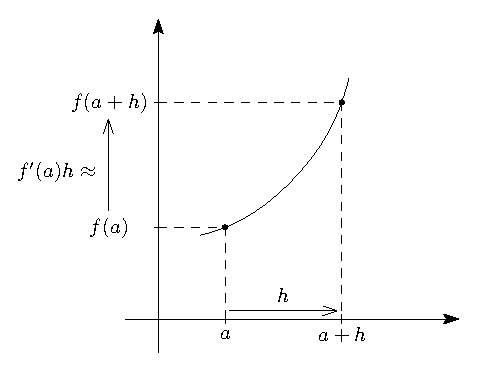
\includegraphics[width=0.45\textwidth]{22_1.eps}
	\caption{Геометрический смысл дифференцируемости.}
	\label{22_1}
\end{figure}

На числовой прямой $h$ представляется как число, в пространстве это будет вектор.

\subsection*{Функция $f(x) = x$}

$f(x) = x \Rightarrow a+h -a = 1{\cdot}h + 0{\cdot}h \Rightarrow dx(h) = h$

$df(h) = f^\prime(a){\cdot}h \wedge dx(h) = h \Rightarrow df(h) = f^\prime(a){\cdot}dx(h) \Rightarrow$ отбросим $h \Rightarrow df = f^\prime(a)dx$ - дифференциал в точке $a$, но чтобы не говорить про конкретную точку пишут просто $df = f^\prime(x)dx$.

Поделим дифференциал $f$ на дифференциал $x \Rightarrow \dfrac{df(h)}{dx(h)} = \dfrac{ f^\prime(a){\cdot}h}{h} = f^\prime(a)$. Можно воспринимать $\dfrac{df}{dx}$ как единый символ или как отношение двух линейных функций.

\begin{prop}
	Если $f$ дифференцируема в точке $a$, то $f$ непрерывна в точке $a$.
\end{prop}
\begin{proof}
	$f(a+h) - f(a) = Ah + \alpha(h)h \xrightarrow[h \to 0]{}0 \Rightarrow x = a + h \Rightarrow \lim\limits_{x\to a} f(x) = f(a) \Rightarrow$ непрерывна в точке $a$.
\end{proof}

\begin{rem}
	Обратное утверждение - не верно.
\end{rem}

\textbf{Пример}: $f(x) = |x|$ всюда непрерывна и не дифференцируема в точке $x = 0$: $\lim\limits_{x \to 0}\frac{|x| - |0|}{x - 0} =\lim\limits_{x \to 0}\frac{|x|}{x}$, но этого предела нет, поскольку пределы справа и слева отличаются.

\begin{figure}[H]
	\centering
	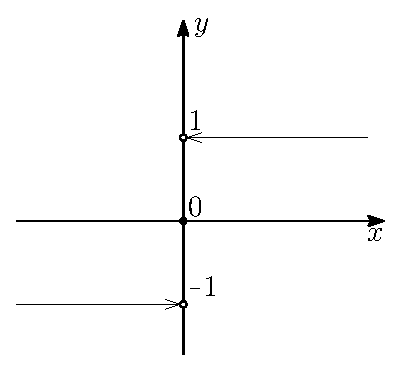
\includegraphics[width=0.3\textwidth]{22_2.eps}
	\caption{Пределы справа и слева у $\frac{|x|}{x}$ различаются.}
	\label{22_2}
\end{figure}

\begin{rem}
	У функции $f(x) = |x|$ нет дифференцируемости только в точке $0$.
\end{rem}

\begin{theorem}\textbf{(Вейрштрасс)}
	Функция $f(x) = \sum\limits_{n=1}^{\infty}2^{-n}\sin(8^nx)$ - непрерывна на $\MR$, но нигде не дифференцируема.
\end{theorem}
\begin{proof}
	При каждом фиксированном $x$ этот ряд сходится, так как он будет ограничен рядом $\sum\limits_{n=1}^{\infty}2^{-n}$.\\
	\textbf{Непрерывность}: Рассмотрим частичные суммы: $S_N(x) = \sum\limits_{n=1}^{N}2^{-n}\sin(8^nx)$. Оценим разность
	$$\Bigg|f(x) - S_N(x)\Bigg| = \Bigg|\sum\limits_{n=N+1}^{\infty}2^{-n}\sin(8^nx)\Bigg|\leq \sum\limits_{n=N+1}^{\infty}2^{-n} = \dfrac{2^{-N-1}}{\tfrac{1}{2}} = 2^{-N}, \forall x \Rightarrow$$
	$$\Rightarrow \sup\limits_{x}|f(x) - S_N(x)| \leq 2^{-N} \xrightarrow[N \to \infty]{} 0$$
	А поскольу $S_N$ это сумма синусов $\Rightarrow S_N$ это непрерывные функции и $S_N$ равномерно сходится к $f \Rightarrow$ \\
	$\Rightarrow f$ - непрерывная функция.
	
	\textbf{Недифференцируемость}: Пусть $x$ - фиксированное, рассмотрим следующее приращение: $f(x\pm2^{-3N-1}\pi) - f(x) = \sum\limits_{n=1}^{\infty}2^{-n}\bigg(\sin(8^n(x\pm \frac{\pi}{2{\cdot}8^N})) - \sin(8^nx)   \bigg)	\Rightarrow$ как только $n > N \Rightarrow$ \\
	$\Rightarrow \sin(8^n(x\pm \frac{\pi}{2{\cdot}8^N}))  - \sin(8^nx) = 0 \Rightarrow f(x\pm2^{-3N-1}\pi) - f(x) = \sum\limits_{n=1}^{N}2^{-n}\bigg(\sin(8^n(x\pm \frac{\pi}{2{\cdot}8^N})) - \sin(8^nx)   \bigg) \Rightarrow$\\
	$\Rightarrow$ поделим на приращение и получим: $\dfrac{f(x\pm2^{-3N-1}\pi) - f(x)}{\pm2^{-3N-1}\pi} = \dfrac{\sum\limits_{n=1}^{N}2^{-n}\bigg(\sin(8^n(x\pm \frac{\pi}{2{\cdot}8^N})) - \sin(8^nx)   \bigg)}{\pm2^{-3N-1}\pi}$.
	
	Оценим последнее слагаемое 
	$$|D_N| = 2^{-N}\Big|\sin(8^Nx\pm \tfrac{\pi}{2}) - \sin(8^Nx)\Big| = 2^{-N}{\cdot}2{\cdot}\Big|\sin\tfrac{\pi}{4}\Big|{\cdot}\Big|\cos(8^Nx \pm \tfrac{\pi}{4})\Big|=2^{-N}{\cdot}2 {\cdot}\frac{1}{\sqrt{2}}{\cdot}\Big|\cos(8^Nx \pm \tfrac{\pi}{4})\Big| $$
	
	\begin{figure}[H]
		\centering
		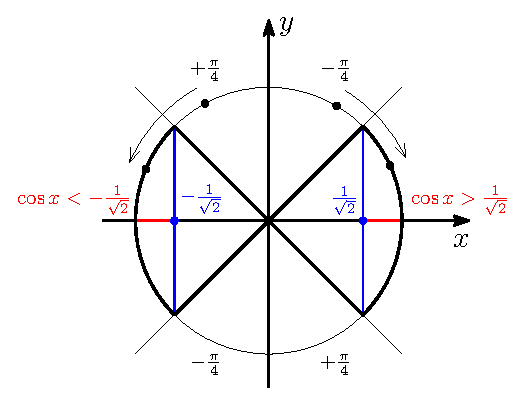
\includegraphics[width=0.55\textwidth]{22_3.eps}
		\caption{Сдвиг по окружности.}
		\label{22_3}
	\end{figure}
			
	Выбирая $+$ или $-$ можем считать (в зависимости от $N$), что $\Big|\cos(8^Nx \pm \tfrac{\pi}{4})\Big| \geq \tfrac{1}{\sqrt{2}} \Rightarrow$ \\
	$$\Rightarrow2^{-N}\Big|\sin(8^Nx\pm \tfrac{\pi}{2}) - \sin(8^Nx)\Big| \geq 2^{-N}$$
	Оценим остальные слагаемые
	$$\Bigg|\sum\limits_{n=1}^{N-1}D_n\Bigg| = \Bigg|\sum\limits_{n=1}^{N-1}2^{-n}\bigg(\sin(8^n(x\pm \tfrac{\pi}{2{\cdot}8^N})) - \sin(8^nx)   \bigg)\Bigg| \leq \sum\limits_{n=1}^{N-1}2^{-n}2\big|\sin(\tfrac{\pi8^n}{4{\cdot}8^N})\big|{\cdot} 1 \underset{|\sin{x}| \leq |x|}{\leq} \sum\limits_{n=1}^{N-1}2^{-n}2\dfrac{\pi8^n}{4{\cdot}8^N} = $$
	$$=\dfrac{\pi}{2{\cdot}8^N}\sum\limits_{n=1}^{N-1}4^n = \dfrac{\pi}{2{\cdot}8^N}{\cdot}\dfrac{4(4^{N-1}-1)}{4-1} \leq \dfrac{\pi 4^N}{2{\cdot}8^N{\cdot}3}=  \dfrac{\pi}{6}2^{-N} < 2^{-N}$$
	
	Таким образом, используя неравенство треугольника $|x| + |y| \geq |x-y|$ получим
	$$\Bigg|\dfrac{f(x\pm2^{-3N-1}\pi) - f(x)}{\pm2^{-3N-1}\pi}\Bigg|	\geq \dfrac{|D_N| - \Bigg|\sum\limits_{n=1}^{N-1}D_n\Bigg|}{2^{-3N-1}\pi} \geq \dfrac{2^{-N} - \tfrac{\pi}{6}2^{-N}}{2^{-3N-1}\pi} = \dfrac{(1 - \tfrac{\pi}{6})}{\pi} 2^{2N+1} \xrightarrow[N \to \infty]{} \infty$$
	Поскольку это верно для любого $x$, то функция нигде не дифференцируема.
\end{proof}

\begin{rem}
	При разных $N$ выбирается правильный знак, то есть $\pm$ зависит от $N$. Это нужно чтобы отношение приращения функции к отношению аргумента стремилось к бесконечности.
\end{rem}

Есть понятие обобщенной производной, там все функции дифференцируемы. Чтобы функция стала недифференцируемой, в текущем понимании, достаточно добавить к ней узкую недифференцируемую $\Rightarrow$ получим недифференцируемую функцию.

\newpage
\section*{Правила дифференцирования}
\begin{enumerate}[label={\arabic*)}]
	\item Если $f$ и $g$ дифференцируемы в точке $a$, то $f+g$ дифференцируема в точке $a$;
	 $$(f+ g)^\prime(a) = f^\prime(a) + g^\prime(a)$$
	 $$d(f+g) = df + dg$$
	 \item \textbf{(Правило Лейбница)}: Если $f$ и $g$ дифф-мы в точке $a$, то $f{\cdot}g$ дифференцируемо в точке $a$;
	 $$(f{\cdot}g)^\prime(a) = f^\prime(a)g(a) + f(a)g^\prime(a)$$
	 $$d(f{\cdot}g)(a,h) = g(a)df(a,h) + f(a)dg(a,h) \Leftrightarrow d(fg) = gdf + fdg$$
	 \item Если $f$ дифференцируема в точке $a$ и $f(a) \neq 0$, то $\dfrac{1}{f}$ дифференцируема в точке $a$
	 $$\bigg(\dfrac{1}{f}\bigg)^\prime(a) = - \dfrac{f^\prime(a)}{f(a)^2}$$ 
	 $$d \dfrac{1}{f} = -\dfrac{1}{f(a)^2}df$$
\end{enumerate}

\begin{proof}\hfill
	\begin{enumerate}[label={\arabic*)}]
		\item $$\lim\limits_{x \to a}\dfrac{f(x) + g(x) - (f(a) + g(a))}{x-a} =\lim\limits_{x \to a}\dfrac{f(x) - f(a)}{x-a} + \lim\limits_{x \to a}\dfrac{g(x) -  g(a)}{x-a} = f^\prime(a) + g^\prime(a)$$
		для дифференциалов аналогично, из определения дифференциалов.
		\item $$\lim\limits_{x \to a}\dfrac{f(x)g(x) - f(a)g(a)}{x-a} = \lim\limits_{x \to a}\dfrac{f(x)g(x) + f(a)g(x) - f(a)g(x) - f(a)g(a)}{x-a} =$$
		$$ =\lim\limits_{x \to a}\dfrac{f(x) - f(a)}{x-a}{\cdot}g(x) + \lim\limits_{x \to a}\dfrac{g(x) -  g(a)}{x-a}{\cdot}f(x) = f^\prime(a)g(a) + g^\prime(a)f(a)$$ поскольку $f$ и $g$ дифференцируемы $\Rightarrow$ они непрерывны. Для дифференциалов аналогично, из определения дифференциалов.
		\item  $$\lim\limits_{x \to a}\dfrac{\frac{1}{f(x)} - \frac{1}{f(a)}}{x-a} = \lim\limits_{x \to a}\dfrac{-1}{f(x)f(a)}{\cdot}\dfrac{f(x) - f(a)}{x-a} = -\dfrac{1}{f(a)^2}{\cdot}f^\prime(a)$$
		поскольку $f(a) \neq 0 \Rightarrow \dfrac{1}{f}$ непрерывна в точке $a$.
	\end{enumerate}
\end{proof}

\begin{theorem}\textbf{(Дифф. сложной функции)}
	Пусть $f \colon \MU(a) \to \MV(f(a)), \, g\colon \MV(f(a)) \to \MR $, \\ 
	где $\MU(a)$ - окрестность точки $a$, $\MV(f(a))$ - окрестность точки $f(a)$ и $f$ - дифференцируема в точке $a$, $g$ - дифференцируема в точке $f(a)$. Тогда $(g \circ f) (x) = g(f(x))$ - дифференцируема в точке $a$ и $$\big( g(f(x))\big)^\prime(a) = g^\prime(f(a)){\cdot}f^\prime(a)$$
\end{theorem}
\begin{proof}\textbf{(Неверное доказательство)}
	$$\lim\limits_{x \to a}\dfrac{g(f(x)) - g(f(a))}{x-a} = \lim\limits_{x \to a}\dfrac{g(f(x)) - g(f(a))}{f(x)-f(a)}{\cdot}\dfrac{f(x) - f(a)}{x-a}$$ 
	Функция $f$ - непрерывная $\Rightarrow f(x) \to f(a)$ при $x \to a \Rightarrow$
	$$\lim\limits_{x \to a}\dfrac{g(f(x)) - g(f(a))}{f(x)-f(a)}{\cdot}\dfrac{f(x) - f(a)}{x-a} = g^\prime(f(a)){\cdot}f^\prime(a)$$
	это не верное доказательство, поскольку мы должны быть уверены, что внутренняя функция не будет заходить в предельную точку для предела композиций двух функций. Необходимо этот момент учитывать, если только это не комбинация двух непрерывных функций, а здесь это не так, поскольку делим на что-то что в точке $a$ обращается в 0. Например, $f(x)$ в точках сколь угодно близких к $a$ может принимать значения равные $f(a)$.
\end{proof}
\begin{proof}\textbf{(Верное доказательство)}
	Так как функция $f$ дифференцируема в точке $a$, то 
	$$f(a+h) - f(a) = f^\prime(a)h + \alpha(h)h \wedge \lim\limits_{h \to 0}\alpha(h) = 0$$ 
	Так как $g$ дифференцируема в точке $f(a)$, то 
	$$g(f(a) + t) - g(f(a)) = g^\prime(f(a))t + \beta(t)t \wedge \lim\limits_{t \to 0}\beta(t) = 0$$
	Определим $\beta(0) = 0 \Rightarrow$ равенство теперь верно $\forall t$ из окрестности $0$, а функция $\beta$ - непрерывна в $0$. Подставим $t = f(a+h) - f(a)$ (раньше не могли, так как раншье можно было подставлять только $t\neq 0$, а это выражение могло оказаться равным $0$) $\Rightarrow$
	$$\Rightarrow g(f(a+h)) - g(f(a)) = g^\prime(f(a)){\cdot}(f(a+h) - f(a)) + \beta(f(a+h) - f(a)){\cdot}(f(a+h) - f(a)) = $$
	$$ = g^\prime(f(a)){\cdot}(f^\prime(a){\cdot}h + \alpha(h){\cdot}h) + \beta(f(a+h) - f(a)){\cdot}(f^\prime(a){\cdot}h + \alpha(h){\cdot}h) = $$
	$$=g^\prime(f(a))f^\prime(a){\cdot}h + \big( g^\prime(f(a))\alpha(h) + \beta(f(a+h) - f(a)){\cdot}(f^\prime(a) + \alpha(h))\big){\cdot}h$$
	Заметим, что $\lim\limits_{h \to 0}g^\prime(f(a))\alpha(h) = 0$, $\lim\limits_{h\to 0}(f^\prime(a) + \alpha(h)) = f^\prime(a)$ и $ \beta(f(a+h) - f(a))$ - композиция двух непрерывных функций $\Rightarrow$ это непрерывная функция и в точке $h = 0$ она будет равна $\beta(0) = 0 \Rightarrow$\\
	$\Rightarrow \lim\limits_{h \to 0} \big( g^\prime(f(a))\alpha(h) + \beta(f(a+h) - f(a)){\cdot}(f^\prime(a) + \alpha(h))\big) = 0$, таким образом
	$$ g(f(a+h)) - g(f(a)) = g^\prime(f(a))f^\prime(a){\cdot}h + \gamma(h){\cdot}h\wedge \lim\limits_{h \to 0}\gamma(h) = 0$$
\end{proof}

\end{document}